\definecolor{cbBlue}{HTML}{0072B2}
\definecolor{cbOrange}{HTML}{E69F00}
\definecolor{cbPurple}{HTML}{CC79A7}

\begin{figure}[ht]
    \centering
    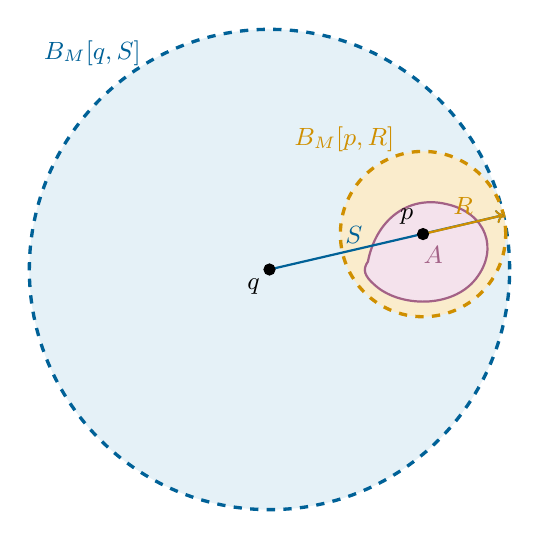
\begin{tikzpicture}[scale=1.0, every node/.style={font=\small}]
        \coordinate (q) at (0,0);
        \coordinate (p) at (1.95,0.45);
        \coordinate (borda) at (2.97,0.69);

        % Bola com centro arbitrario q.
        \path[fill=cbBlue!10] (q) circle (3.05);
        \draw[cbBlue!85!black, very thick, dashed] (q) circle (3.05);
        \node[cbBlue!85!black] at (-2.25,2.75) {$B_M[q,S]$};

        % Bola que contem o conjunto limitado.
        \path[fill=cbOrange!20] (p) circle (1.05);
        \draw[cbOrange!90!black, very thick, dashed] (p) circle (1.05);
        \node[cbOrange!90!black] at (0.95,1.65) {$B_M[p,R]$};

        % Conjunto A.
        \path[fill=cbPurple!22]
            (1.25,0.1)
            .. controls (1.35,0.62) and (1.75,0.95) .. (2.25,0.83)
            .. controls (2.75,0.72) and (2.92,0.26) .. (2.62,-0.12)
            .. controls (2.32,-0.5) and (1.65,-0.48) .. (1.34,-0.2)
            .. controls (1.2,-0.08) and (1.18,0.0) .. (1.25,0.1)
            -- cycle;
        \draw[cbPurple!80!black, thick]
            (1.25,0.1)
            .. controls (1.35,0.62) and (1.75,0.95) .. (2.25,0.83)
            .. controls (2.75,0.72) and (2.92,0.26) .. (2.62,-0.12)
            .. controls (2.32,-0.5) and (1.65,-0.48) .. (1.34,-0.2)
            .. controls (1.2,-0.08) and (1.18,0.0) .. (1.25,0.1)
            -- cycle;
        \node[cbPurple!80!black] at (2.08,0.18) {$A$};

        % Centros e raios.
        \draw[cbBlue!85!black, thick, ->] (q) -- (borda)
            node[pos=0.28, above right] {$S$};
        \draw[cbOrange!90!black, thick, ->] (p) -- (borda)
            node[midway, above] {$R$};

        \filldraw[black] (p) circle (2pt) node[above left] {$p$};
        \filldraw[black] (q) circle (2pt) node[below left] {$q$};
    \end{tikzpicture}
    \caption{Um conjunto limitado contido em bolas com centros distintos.}
    \label{fig:centroConjuntoLimitado}
\end{figure}
